\section{Запись разрешающей системы уравнений МКЭ, проведение ее анализа и получение <<вручную>> решения для перемещений и напряжений}

Разрешающую систему МКЭ получим методом равновесия узлов. Для этого составим дискретную модель. За конечный элемент возьмем каждый участок длиной $l$:
\begin{figure}[H]
    \begin{center}
        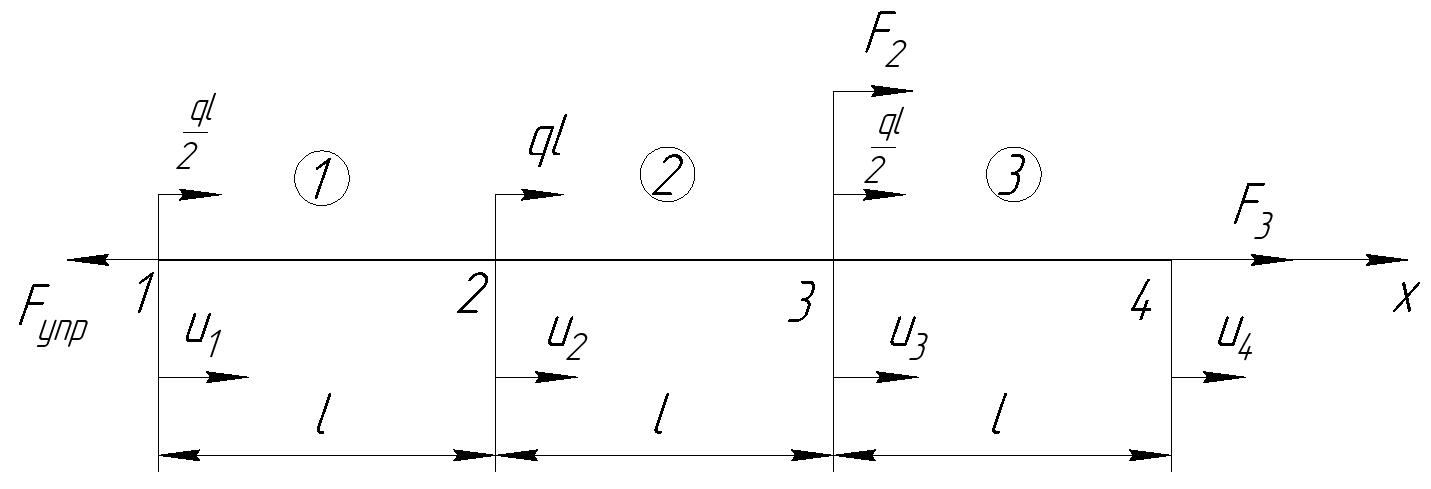
\includegraphics[width = 0.7\linewidth]{pic6.1.PNG}
        \caption{Дискретная модель}
        \label{pic6.1}
    \end{center}
\end{figure}

Разрежем модель на конечные элемнты и узлы:
\begin{figure}[H]
    \begin{center}
        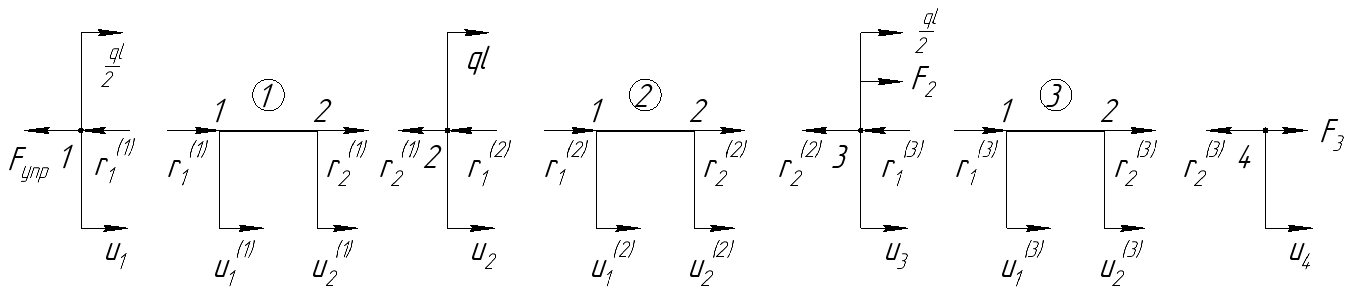
\includegraphics[width = \linewidth]{pic6.2.PNG}
        \caption{Разбиение дискретной модели на узлы и КЭ}
        \label{pic6.2}
    \end{center}
\end{figure}

Запишем условие равновесия для i-го КЭ:
\begin{equation}
    \label{eq6.1}
    \frac{EF}{l}
    \begin{bmatrix}
        1 & -1
        \\
        -1 & 1
    \end{bmatrix}
    \begin{Bmatrix}
        u_{1}^{(i)}
        \\
        u_{2}^{(i)}
    \end{Bmatrix}
    = 
    \begin{Bmatrix}
        r_{1}^{(i)}
        \\
        r_{2}^{(i)}
    \end{Bmatrix}
\end{equation}
или в обычном виде:
\begin{equation}
    \label{eq6.2}
    \begin{cases}
        \displaystyle \frac{EF}{l} (u_1^{(i)} - u_2^{(i)}) = r_1^{(i)}
        \\[10pt]
        \displaystyle \frac{EF}{l} (u_2^{(i)} - u_1^{(i)}) = r_2^{(i)}
    \end{cases}
\end{equation}

Запишем условия равновесия узлов:
\begin{equation}
    \label{eq6.3}
    \begin{cases}
        \displaystyle F_{\t{упр}} + r_1^{(1)} - \frac{ql}{2} = 0
        \\
        \displaystyle r_2^{(1)} + r_1^{(2)} - ql = 0
        \\
        \displaystyle r_2^{(2)} + r_1^{(3)} - F_2 - \frac{ql}{2} = 0
        \\
        \displaystyle r_2^{(3)} - F_3 = 0
    \end{cases}
\end{equation}

Подставим (\ref{eq6.2}) в (\ref{eq6.3}) и учтем, что $F_{\t{упр}} = c \cdot u_1$:
\begin{equation}
    \label{eq6.4}
    \begin{cases}
        \displaystyle cu_1 + \frac{EF}{l} (u_1^{(1)} - u_2^{(1)}) - \frac{ql}{2} = 0
        \\[10pt]
        \displaystyle \frac{EF}{l} (u_2^{(1)} - u_1^{(1)}) + \frac{EF}{l} (u_1^{(2)} - u_2^{(2)}) - ql = 0
        \\[10pt]
        \displaystyle \frac{EF}{l} (u_2^{(2)} - u_1^{(2)}) + \frac{EF}{l} (u_1^{(3)} - u_2^{(3)}) - F_2 - \frac{ql}{2} = 0
        \\[10pt]
        \displaystyle \frac{EF}{l} (u_2^{(3)} - u_1^{(3)}) - F_3 = 0
    \end{cases}
\end{equation}

Объединим все элементы в единую систему. Тогда будут выполняться следующие соотношения:
\begin{equation}
    \label{eq6.5}
    \begin{cases}
        u_1^{(1)} = u_1
        \\
        u_2^{(1)} = u_1^{(2)} = u_2
        \\
        u_2^{(2)} = u_1^{(3)} = u_3
        \\
        u_2^{(3)} = u_4
    \end{cases}
\end{equation}

Подставим (\ref{eq6.5}) в (\ref{eq6.4}):
\begin{equation}
    \label{eq6.6}
    \begin{cases}
        \displaystyle cu_1 + \frac{EF}{l} (u_1 - u_2) - \frac{ql}{2} = 0
        \\[10pt]
        \displaystyle \frac{EF}{l} (u_2 - u_1) + \frac{EF}{l} (u_2 - u_3) - ql = 0
        \\[10pt]
        \displaystyle \frac{EF}{l} (u_3 - u_2) + \frac{EF}{l} (u_3 - u_4) - F_2 - \frac{ql}{2} = 0
        \\[10pt]
        \displaystyle \frac{EF}{l} (u_4 - u_3) - F_3 = 0
    \end{cases}
\end{equation}

Сгруппируем коэффициенты при одинаковых перемещениях и перенесем нагрузку в правую часть:
\begin{equation}
    \label{eq6.7}
    \begin{cases}
        \displaystyle (c + \frac{EF}{l}) u_1 - \frac{EF}{l} u_2 = \frac{ql}{2}
        \\[10pt]
        \displaystyle - \frac{EF}{l} u_1 + 2 \frac{EF}{l} u_2 - \frac{EF}{l} u_3 = ql
        \\[10pt]
        \displaystyle - \frac{EF}{l} u_2 + 2 \frac{EF}{l} u_3 - \frac{EF}{l} u_4 = F_2 + \frac{ql}{2}
        \\[10pt]
        \displaystyle - \frac{EF}{l} u_3 + \frac{EF}{l} u_4 = F_3
    \end{cases}
\end{equation}

Запишем (\ref{eq6.7}) в матричном виде:
\begin{equation}
    \label{eq6.8}
    \begin{bmatrix}
        c + \matrfrac{EF}{l} & - \matrfrac{EF}{l} & 0 & 0
        \\[10pt]
        - \matrfrac{EF}{l} & 2 \matrfrac{EF}{l} & - \matrfrac{EF}{l} & 0
        \\[10pt]
        0 & - \matrfrac{EF}{l} & 2 \matrfrac{EF}{l} & - \matrfrac{EF}{l}
        \\[10pt]
        0 & 0 & - \matrfrac{EF}{l} & \matrfrac{EF}{l}
    \end{bmatrix}
    \cdot
    \begin{Bmatrix}
        u_1
        \\[10pt]
        u_2
        \\[10pt]
        u_3
        \\[10pt]
        u_4
    \end{Bmatrix}
    =
    \begin{Bmatrix}
        \matrfrac{ql}{2}
        \\[10pt]
        ql
        \\[10pt]
        F_2 + \matrfrac{ql}{2}
        \\[10pt]
        F_3
    \end{Bmatrix}
\end{equation}
Разделим (\ref{eq6.8}) на $\displaystyle \frac{EF}{l}$ учитывая (\ref{eq0.1}):
\begin{equation}
    \label{eq6.9}
    \begin{bmatrix}
        8 & -1 & 0 & 0
        \\
        -1 & 2 & -1  & 0
        \\
        0 & -1 & 2 & -1
        \\
        0 & 0 & -1 & 1
    \end{bmatrix}
    \cdot
    \begin{Bmatrix}
        u_1
        \\
        u_2
        \\
        u_3
        \\
        u_4
    \end{Bmatrix}
    =
    \begin{Bmatrix}
        \displaystyle \frac{l}{2}
        \\
        l
        \\
        l
        \\
        0.2l
    \end{Bmatrix}
\end{equation}

Искать решения для системы (\ref{eq6.9}) будем методом Крамера:
\begin{equation}
    \label{eq6.10}
    u_i = \frac{\Delta_i}{\Delta}
\end{equation}
\begin{equation}
    \label{eq6.11}
    \begin{split}
        & \Delta =
        \begin{vmatrix}
            8 & -1 & 0 & 0
            \\
            -1 & 2 & -1 & 0
            \\
            0 & -1 & 2 & -1
            \\
            0 & 0 & -1 & 1
        \end{vmatrix}
        = 8 \cdot
        \begin{vmatrix}
            2 & -1 & 0
            \\
            -1 & 2 & -1
            \\
            0 & -1 & 1
        \end{vmatrix}
        + 1 \cdot
        \begin{vmatrix}
            -1 & -1 & 0
            \\
            0 & 2 & -1
            \\
            0 & -1 & 1
        \end{vmatrix}
        =
        \\
        & = 8 \cdot [2 \cdot (2-1) + 1(-1)] + (-1)(2-1) + 1 \cdot 0 = 8 - 1 = 7
    \end{split}
\end{equation}
\begin{equation}
    \label{eq6.12}
    \begin{split}
        & \Delta_1 = 
        \begin{vmatrix}
            \displaystyle \frac{l}{2} & -1 & 0 & 0
            \\
            l & 2 & -1 & 0
            \\
            l & -1 & 2 & -1
            \\
            0.2l & 0 & -1 & 1
        \end{vmatrix}
        = \frac{l}{2} [ 2 \cdot (2 - 1) + 1 \cdot (-1) ] + 1 \cdot [l \cdot (2 - 1) + 1 \cdot (l + 0.2l)] = 
        \\
        & = 0.5l + 2.2l = 2.7l
    \end{split}
\end{equation}
\begin{equation}
    \label{eq6.13}
    \begin{split}
        & \Delta_2 = 
        \begin{vmatrix}
            8 & \displaystyle \frac{l}{2} & 0 & 0
            \\
            -1 & l & -1 & 0
            \\
            0 & l & 2 & -1
            \\
            0 & 0.2l & -1 & 1
        \end{vmatrix}
        = 8 \cdot [l \cdot (2 - 1) + 1 \cdot (l + 0.2l)] - 0.5l \cdot [-1 \cdot (2 - 1) + 1 \cdot (0)] =
        \\
        & = 8 \cdot (l + 1.2l) - 0.5l \cdot (-1) = 18.1l
    \end{split}
\end{equation}
\begin{equation}
    \label{eq6.13.1}
    \begin{split}
        & \Delta_3 =
        \begin{vmatrix}
            8 & -1 & \displaystyle \frac{l}{2} & 0
            \\
            -1 & 2 & l & 0
            \\
            0 & -1 & l & -1
            \\
            0 & 0 & 0.2l & 1
        \end{vmatrix}
        = -0.2l \cdot [1 \cdot 0 - 1 \cdot (8 \cdot 2 - 1)] + 1 \cdot [1 \cdot (8l + 0.5l) + l \cdot (8 \cdot 2 - 1)] = 
        \\
        & = -0.2l \cdot (-15) + 8.5l + 15l = 26.5l
    \end{split}
\end{equation}
\begin{equation}
    \label{eq6.13.2}
    \begin{split}
        & \Delta_4 =
        \begin{vmatrix}
            8 & -1 & 0 & \displaystyle \frac{l}{2}
            \\
            -1 & 2 & -1 & l
            \\
            0 & -1 & 2 & l
            \\
            0 & 0 & -1 & 0.2l
        \end{vmatrix}
        = 1 \cdot [1 \cdot (8l + 0.5l) + l \cdot (8 \cdot 2 - 1)] + 0.2l \cdot [1 \cdot (-8) + 2 \cdot (8 \cdot 2 - 1)] =
        \\
        & = 8.5l + 15l + 0.2l \cdot 22 = 27.9l
    \end{split}
\end{equation}
\begin{equation}
    \label{eq6.14}
    \begin{cases}
        \displaystyle u_1 = \frac{\Delta_1}{\Delta} = 0.386l = 0.193 \; \t{м}
        \\[10pt]
        \displaystyle u_2 = \frac{\Delta_2}{\Delta} = 2.59l = 1.295 \; \t{м}
        \\[10pt]
        \displaystyle u_3 = \frac{\Delta_3}{\Delta} = 3.786l = 1.893 \; \t{м}
        \\[10pt]
        \displaystyle u_4 = \frac{\Delta_4}{\Delta} = 3.986l = 1.993 \; \t{м}
    \end{cases}
\end{equation}

Напряжения вычислим по закону Гука:
\begin{equation}
    \label{eq6.15}
    \sigma_i = E \epsilon_i = E \cdot \frac{u_2^{(i)} - u_1^{(i)}}{l}
\end{equation}
\begin{equation}
    \label{eq6.16}
    \begin{cases}
        \displaystyle \sigma_1 = E \frac{u_2 - u_1}{l} = 2.2E = 1.608 \cdot 10^{11} \; \t{Па}
        \\[10pt]
        \displaystyle \sigma_2 = E \frac{u_3 - u_2}{l} = 1.2E = 8.772 \cdot 10^{10} \; \t{Па} 
        \\[10pt]
        \displaystyle \sigma_3 = E \frac{u_4 - u_3}{l} = 0.2E = 1.462 \cdot 10^{10} \; \t{Па}
    \end{cases}
\end{equation}

\section{Расчет заданной конструкции с использованием пакета MSC Patran\_Nastran}

\section{Сравнительный анализ результатов, полученных методами, использованными в работе}